%%
%% Automatically generated file from DocOnce source
%% (https://github.com/hplgit/doconce/)
%%
%%
% #ifdef PTEX2TEX_EXPLANATION
%%
%% The file follows the ptex2tex extended LaTeX format, see
%% ptex2tex: http://code.google.com/p/ptex2tex/
%%
%% Run
%%      ptex2tex myfile
%% or
%%      doconce ptex2tex myfile
%%
%% to turn myfile.p.tex into an ordinary LaTeX file myfile.tex.
%% (The ptex2tex program: http://code.google.com/p/ptex2tex)
%% Many preprocess options can be added to ptex2tex or doconce ptex2tex
%%
%%      ptex2tex -DMINTED myfile
%%      doconce ptex2tex myfile envir=minted
%%
%% ptex2tex will typeset code environments according to a global or local
%% .ptex2tex.cfg configure file. doconce ptex2tex will typeset code
%% according to options on the command line (just type doconce ptex2tex to
%% see examples). If doconce ptex2tex has envir=minted, it enables the
%% minted style without needing -DMINTED.
% #endif

% #define PREAMBLE

% #ifdef PREAMBLE
%-------------------- begin preamble ----------------------

\documentclass[%
oneside,                 % oneside: electronic viewing, twoside: printing
final,                   % draft: marks overfull hboxes, figures with paths
10pt]{article}

\listfiles               % print all files needed to compile this document

\usepackage{relsize,makeidx,color,setspace,amsmath,amsfonts,amssymb}
\usepackage[table]{xcolor}
\usepackage{bm,microtype}

\usepackage[pdftex]{graphicx}

\usepackage[T1]{fontenc}
%\usepackage[latin1]{inputenc}
\usepackage{ucs}
\usepackage[utf8x]{inputenc}

\usepackage{lmodern}         % Latin Modern fonts derived from Computer Modern

% Hyperlinks in PDF:
\definecolor{linkcolor}{rgb}{0,0,0.4}
\usepackage{hyperref}
\hypersetup{
    breaklinks=true,
    colorlinks=true,
    linkcolor=linkcolor,
    urlcolor=linkcolor,
    citecolor=black,
    filecolor=black,
    %filecolor=blue,
    pdfmenubar=true,
    pdftoolbar=true,
    bookmarksdepth=3   % Uncomment (and tweak) for PDF bookmarks with more levels than the TOC
    }
%\hyperbaseurl{}   % hyperlinks are relative to this root

\setcounter{tocdepth}{2}  % number chapter, section, subsection

% Tricks for having figures close to where they are defined:
% 1. define less restrictive rules for where to put figures
\setcounter{topnumber}{2}
\setcounter{bottomnumber}{2}
\setcounter{totalnumber}{4}
\renewcommand{\topfraction}{0.95}
\renewcommand{\bottomfraction}{0.95}
\renewcommand{\textfraction}{0}
\renewcommand{\floatpagefraction}{0.75}
% floatpagefraction must always be less than topfraction!
% 2. ensure all figures are flushed before next section
\usepackage[section]{placeins}
% 3. enable begin{figure}[H] (often leads to ugly pagebreaks)
%\usepackage{float}\restylefloat{figure}

% newcommands for typesetting inline (doconce) comments
\newcommand{\shortinlinecomment}[3]{{\color{red}{\bf #1}: #2}}
\newcommand{\longinlinecomment}[3]{{\color{red}{\bf #1}: #2}}

% prevent orhpans and widows
\clubpenalty = 10000
\widowpenalty = 10000

% --- end of standard preamble for documents ---


% insert custom LaTeX commands...

\raggedbottom
\makeindex

%-------------------- end preamble ----------------------

\begin{document}

% endif for #ifdef PREAMBLE
% #endif


% ------------------- main content ----------------------



% ----------------- title -------------------------

\thispagestyle{empty}

\begin{center}
{\LARGE\bf
\begin{spacing}{1.25}
FFM232, Klassisk fysik och vektorfält - Föreläsningsanteckningar
\end{spacing}
}
\end{center}

% ----------------- author(s) -------------------------

\begin{center}
{\bf \href{{http://fy.chalmers.se/subatom/tsp/}}{Christian Forssén}, Institutionen för fysik, Chalmers, Göteborg, Sverige${}^{}$} \\ [0mm]
\end{center}

\begin{center}
% List of all institutions:
\end{center}
    
% ----------------- end author(s) -------------------------

% --- begin date ---
\begin{center}
Oct 3, 2016
\end{center}
% --- end date ---

\vspace{1cm}


\section{9. Lösningar av Poissons ekvation}

Vi vet att Poissons ekvation
$$
\Delta \phi(\vec{r}) = - \rho(\vec{r}),
$$
har entydiga lösningar om
\begin{align}
\phi|_{\partial V} &= f(\vec{r}) \quad & \mathrm{Dirichlets~randvillkor} \nonumber \\
(\nabla\phi)|_{\partial V} \cdot \vec{n} &= g(\vec{r}) \quad & \mathrm{Neumans~randvillkor} \nonumber 
\end{align}
där $f$ och $g$ är funktioner på randen $\partial V$.

\subsection{Lösning av Poissons ekvation}

Vi kommer att betrakta fyra olika lösningsmetoder:

\paragraph{1. Greensfunktionsmetoden.}
\paragraph{2. Spegling.}
\paragraph{3. Variabelseparation.}
\paragraph{4. Numeriska metoder.}
\begin{itemize}
\item De tre förstnämnda är analytiska metoder som vi introducerar för att ge en fysikalisk förståelse av lösningarna.

\item De numeriska metoderna är förstås viktigast för praktiska tillämpningar. Se datoruppgift.
\end{itemize}

\noindent
\subsection{1. Greensfunktionsmetoden}

Vi skall här titta på lösningar till Poissons ekvation,
$$
\Delta\phi(\vec{r})=-\rho(\vec{r}).
$$ 
Vi begränsar oss till homogena randvillkor, dvs.~$f,g=0$ på randen.

Lös först (med randvillkor!)
$$
\Delta G(\vec{r},\vec{r}{\;}') = -\delta(\vec{r} - \vec{r}{\;}'),
$$
dvs för en punktkälla i $\vec{r} = \vec{r}{\;}'$ med $q=1$. 

\longinlinecomment{Comment 1}{ Notera att Laplaceoperatorn verkar på variabeln $\vec{r}$ (inte $\vec{r}{\;}'$). Dvs., $\Delta = \Delta_{\vec{r}} = \partial_x^2 + \partial_y^2 + \partial_z^2$. }{ Notera att Laplaceoperatorn verkar }

Källfördelningen $\rho$ kan skrivas som en superposition
$$
\rho(\vec{r})=\int_{V'}\mbox{d}V'\,\delta^3(\vec{r}-\vec{r}{\;}')\rho(\vec{r}{\;}').
$$
Lösningen blir en superposition av Greensfunktioner
$$
\phi(\vec{r})=\int_{V'}\mbox{d}V'\,G(\vec{r},\vec{r}{\;}')\rho(\vec{r}{\;}').
$$
Detta visas genom insättning:
\begin{align}
\Delta\phi(\vec{r}) &= \Delta\int_{V'}\mbox{d}V'\,G(\vec{r},\vec{r}{\;}')\rho(\vec{r}{\;}')
=\int_{V'}\mbox{d}V'\,\Delta G(\vec{r},\vec{r}{\;}')\rho(\vec{r}{\;}') \nonumber \\
&=-\int_{V'}\mbox{d}V'\,\delta^3(\vec{r}-\vec{r}{\;}')\rho(\vec{r}{\;}')
=-\rho(\vec{r}).
\end{align}

\begin{itemize}
\item Notera att Greensfunktionen $G$ på ett område $V$ bestäms av formen på området och av randvillkoren på $\partial V$.

\item På $\mathbf{R}^3$ är Greensfunktionen
\end{itemize}

\noindent
$$
G(\vec{r},\vec{r}{\;}')=\frac{1}{4\pi|\vec{r}-\vec{r}{\;}'|},
$$
och lösningen till Poissons ekvation med källa $\rho$ blir
$$
\phi(\vec{r})=\int_{\mathbf{R}^3}\mbox{d}V'\,\frac{\rho(\vec{r}{\;}')}{4\pi|\vec{r}-\vec{r}{\;}'|}.
$$
\shortinlinecomment{Comment 2}{ Detta är förstås samma uttryck som vi härledde genom superposition i kapitel 6. }{ Detta är förstås samma }

---------------------------------------------------------
\paragraph{Exempel: linjekälla.}


\vspace{3mm}


Betrakta en linjekälla, $\rho(\vec{r})=k\delta^2(\vec{\rho})$, i $\mathbf{R}^3$.

Vi skall integrera över linjekällan och introducerar koordinaten
$$
\vec{r}{\;}' = \vec{\rho}{\;}' + z' \hat{z}' = \rho' \hat{\rho}' + z' \hat{z},
$$
där vi noterar att det inte behövs något ``prim'' på $z$-riktningen.

Vi sätter in i 
$$
\phi(\vec{r}) = \int_{\mathbf{R}^3}\rho(\vec{r}{\;}')G(\vec{r},\vec{r}{\;}')\mbox{d}V'
=\int_{-\infty}^{\infty}dz'\int_{\mathbf{R}^2}dS'
       \frac{k\delta^2(\vec{\rho}{\;}')}{4\pi|\vec{r}-(\rho'\hat\rho{}'+z'\hat z)|} .
$$

Integralen $\int dS'$ över $x'$ och $y'$ kan enkelt utföras tack vare deltafunktionen. Resultatet:
$$
\phi(\vec{r})=\int_{-\infty}^{\infty}dz' \frac{k}{4\pi|\vec{r}-z'\hat z|}
$$  
som är identiskt med den direkta konstruktionen från kap. 6.

---------------------------------------------------------
\paragraph{Exempel: virveltråd.}


\vspace{3mm}


Poissons ekvation för ett vektorfält,
$$
\Delta\vec A = -\vec\jmath, 
$$
Divergensfritt fält $\vec B$ som därmed kan uttryckas som rotationen av en
vektorpotential, $\vec B=\nabla\times\vec A$. 

Lösningen blir
$$
\vec A(\vec{r})=\int_{\mathbf{R}^3} \mbox{d}V'\, \frac{\vec\jmath(\vec{r}{\;}')}{4\pi|\vec{r}-\vec{r}{\;}'|}.
$$
Av speciellt intresse är en virveltråd med konstant styrka $J$ längs en oändlig eller sluten kurva $C$. Virveltätheten blir $\vec{jmath}(\vec{r}{\;}') = J \delta^2(\vec{\rho}{\;}') \mbox{d}\vec{r}{\;}' / \mbox{d}r'$, dvs den är riktad längs kurvan $C$, där vektorn $\vec{\rho}{\;}'$ är vinkelrät mot kurvan. Vektorpotentialen blir
$$
\vec A(\vec{r})=\int_C \frac{J \mbox{d}\vec{r}{\;}'}{4\pi|\vec{r}-\vec{r}{\;}'|},
$$
där vi kan utföra volymsintegralen över $\mbox{d}r'\mbox{d}\vec{\rho}{\;}'$, dvs en riktning längs kurvan $C$ och en yta vinkelrät mot densamma.

Resultatet motsvarar t.ex. den EM vektorpotentialen från en tunn elektrisk ledare med strömmen $J$.

---------------------------------------------------------

\subsection{2. Spegling}

\begin{itemize}
\item Vi såg att lösningen $\phi(\vec{r})$ erhålls enkelt om man har tillgång till Greensfunktionen. Men denna är ofta svår att finna. 

\item För vissa geometrier erbjuder \emph{speglingsmetoden} ett väldigt elegant sätt att konstruera Greensfunktionen.
\end{itemize}

\noindent
Betrakta halvrymden $\{\vec{r}:\,z>0\}$ med ett homogent randvillkor på planet
$z=0$: 
\begin{itemize}
\item Dirichlets randvillkor: $\phi=0$, eller 

\item Neumanns, $\frac{\partial \phi}{\partial z} = 0$.
\end{itemize}

\noindent
\longinlinecomment{Comment 3}{ Detta är ett bra tillfälle att repetera begreppen ekvipotentialytor och fältlinjer (till vektorfältet $-\nabla\phi$). Se till att förstå att ett randvillkor $\phi=0$ (Dirichlet) betyder att randen är en ekvipotentialyta, och att $\vec n \cdot \nabla\phi=0$ betyder att fältlinjerna är parallella med randen. }{ Detta är ett bra }



% inline figure
\centerline{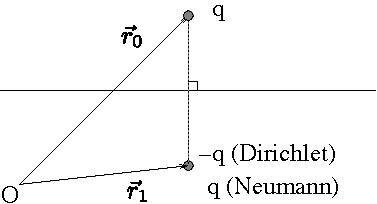
\includegraphics[width=0.5\linewidth]{fig/spegling.pdf}}



\begin{itemize}
\item Spegelladdningen finns i ett område som vi inte är intresserade av ($z<0$), men hjälper till att uppfylla randvillkoren.
\end{itemize}

\noindent
Med $\vec{r}_0 = (x_0,y_0,z_0)$ och $\vec{r}_1 = (x_0,y_0,-z_0)$ och:
\begin{itemize}
\item $q_1 = q$ uppfylls Neumanns randvillor

\item $q_1 = -q$ uppfylls Dirichlets randvillor
\end{itemize}

\noindent
dvs potentialen från den två punktladdningarna
$$
\phi(\vec{r}) = \frac{q}{4 \pi |\vec{r} - \vec{r}_0|} \pm \frac{q}{4 \pi |\vec{r} - \vec{r}_1|}
$$
I det förra fallet är fältlinjerna parallella med $z=0$ planet, i det senare fallet ligger ekvipotentialytan $\phi=0$ i $z=0$ planet.

Greensfunktionen med Dirichlets homogena randvillkor blir här alltså
$$
G (\vec{r},\vec{r}_0)=\frac{1}{4\pi|\vec{r}-\vec{r}_0|} - \frac{1} {4\pi|\vec{r}-\vec{r}_1|}.
$$

\longinlinecomment{Comment 4}{ Notera att $G(\vec{r},\vec{r}_0)$ uppfyller $\Delta G(\vec{r},\vec{r}_0) = - \delta(\vec{r}-\vec{r}_0)$ i det övre halvrummet. }{ Notera att $G(\vec{r},\vec{r}_0)$ uppfyller }

Intressant nog fungerar speglingsmetoden även för cirklar i två dimensioner och sfärer i tre dimensioner (i det senare fallet dock endast för Dirichlets randvillkor). Se demonstrationsuppgift.



% inline figure
\centerline{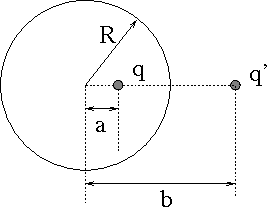
\includegraphics[width=0.5\linewidth]{fig/spegling2.pdf}}



\subsection{3. Variabelseparation}

\begin{itemize}
\item Bygger på att man löser ekvationerna stegvis i en variabel i taget. 

\item Problemet skall \emph{passa bra} ihop med ett visst koordinatsystem.
\end{itemize}

\noindent
---------------------------------------------------------

\paragraph{Exempel: Laplaces ekvation på en cirkelskiva.}


\vspace{3mm}


\begin{itemize}
\item $\Delta\phi=0$, på $\varrho=\sqrt{x^2+y^2}<a$. 

\item Betrakta fallet där randvillkoret enbart innehåller ett vinkelberoende
\end{itemize}

\noindent
$$
\left. \phi(\vec{r}) \right|_{\partial V} = h(\varphi)
$$

Laplaceoperatorn är
$$
\Delta = \frac{1}{\varrho} \frac{\partial}{\partial \varrho} \varrho \frac{\partial}{\partial \varrho} +
 \frac{1}{\varrho^2} \frac{\partial^2}{\partial \varphi^2}.
$$
Vi kan lösa ekvationen genom att separera beroendet på variabeln $\varphi$ och
$\varrho$. 

\paragraph{Specialfall.}
Antag att randvillkoret är
$$
\phi(a,\varphi)=\phi_0\cos m\varphi,
$$ 
där $m$ är ett heltal.

Vi ansätter att hela lösningen har just detta beroende av $\varphi$, så att 
$$
\phi(\varrho)=f(\varrho)\cos m\varphi
$$
Funktionen $\cos m\varphi$ uppfyller 
$$
\frac{\partial ^2}{\partial \varphi^2} \cos m\varphi = -m^2 \cos m\varphi,
$$
dvs.~den är en egenfunktion till $\frac{\partial^2}{\partial \varphi^2}$ med egenvärdet $-m^2$. 

Insättning:
$$
\frac{1}{\varrho} \frac{\mbox{d}}{\mbox{d}\varrho} \left( \varrho \frac{\mbox{d}f(\varrho)}{\mbox{d}\varrho} \right) \cos m \varphi - \frac{m^2}{\varrho^2}f(\varrho)\cos m\varphi=0,
$$
och om detta skall gälla överallt på cirkelskivan måste man ha
$$
\varrho \frac{\mbox{d}}{\mbox{d}\varrho} \left(\varrho \frac{\mbox{d}f(\varrho)}{\mbox{d}\varrho} \right)
-m^2f(\varrho)=0.
$$
Den partiella differentialekvationen har nu reducerats till en ordinär differentialekvation.

\begin{itemize}
\item Ansatz: $f(\varrho)=A\varrho^p$ 

\item Löser ekvationen med $p^2-m^2=0$, dvs.~$p=\pm m$, där minustecknet väljs bort på grund av singulariteten i origo. 

\item Slutsats:
\end{itemize}

\noindent
$$
\phi(\varrho,\varphi)=\phi_0\left( \frac{\varrho}{a}\right)^m \cos m\varphi,
$$
är en lösning till Laplaces ekvation på cirkelskivan med randvillkoret $\phi(a,\varphi)=\phi_0\cos m\varphi$.

\paragraph{Mer allmänt randvillkor.}
Med randvillkoret
$$
\phi(a,\varphi)=h(\varphi),
$$
ansätter vi lösningen $\phi(\varrho,\varphi) = f(\varrho) g(\varphi)$.

Laplacianen blir
$$
\Delta \phi = \Delta \left( f(\varrho) g(\varphi) \right) = g(\varphi) \frac{1}{\varrho} \frac{\partial}{\partial\varrho} \left( \varrho \frac{\partial f(\varrho)}{\partial\varrho} \right) + \frac{f(\varrho)}{\rho^2} \frac{\partial^2 g}{\partial\varphi^2} = 0.
$$
Detta ger den \emph{separerade} ekvationen
$$
\frac{f(\varrho) g(\varphi)}{\varrho^2} \left[ \frac{\varrho^2}{f(\varrho)} \frac{1}{\varrho} \frac{\partial}{\partial\varrho} \left( \varrho \frac{\partial f(\varrho)}{\partial\varrho} \right) + \frac{1}{g(\varphi)} \frac{\partial^2 g}{\partial\varphi^2} \right] = 0,
$$
där den första termen i hakparantesen enbart beror på $\varrho$ och den andra bara på $\varphi$. Därmed måste bägge vara konstanta (för att gälla för alla $\varrho,\varphi$). Vi sätter den första till $-\lambda$ och den andra till $+\lambda$.

Studera vinkelekvationen först
$$
\frac{\partial^2 g}{\partial\varphi^2} = \lambda g(\varphi),
$$
dvs vi kan tolka $g$ som en egenfunktion till $\partial^2 / \partial\varphi^2$. Lösningen är
$$
g(\varphi) = A \cos (m \varphi) + B \sin (m \varphi),
$$
med \emph{egenvärdet} $\lambda = -m^2$. Funktionen måste uppfylla randvillkoret $g(0) = g(2\pi)$ vilket ger att $m = 0,1,2,\ldots$ (notera att $m=0$ är meningslös för sinus-termen).

Den kvarvarande, radiella ekvationen blir nu
$$
\frac{1}{\varrho} \frac{\partial}{\partial\varrho} \left( \varrho \frac{\partial f(\varrho)}{\partial\varrho} \right) - \frac{m^2}{\varrho^2} f(\varrho) = 0.
$$

\begin{itemize}
\item $m=0$, vilket innebär att $g(\varphi) = A$
\end{itemize}

\noindent
$$
\frac{\partial}{\partial\varrho} \left( \varrho \frac{\partial f(\varrho)}{\partial\varrho} \right) = 0 \quad \Rightarrow \quad
\varrho \frac{\partial f(\varrho)}{\partial\varrho} = B \quad \Rightarrow \quad
\frac{\partial f(\varrho)}{\partial\varrho} = B \varrho.
$$
Med lösningen $f(\varrho) = A + B \ln(\varrho)$, där den andra termen motsvarar en punktkälla i två dimensioner (vi skippar denna).

Alltså är $\phi(\vec{r}) = A$ (konstant) en lösning om randvillkoret är $h(\varphi) = A$ (konstant).

\begin{itemize}
\item $m > 0$, ansätt lösning $f(\varrho) = C \varrho^p$
\end{itemize}

\noindent
$$
\frac{1}{\varrho} \frac{\partial}{\partial\varrho} \left( \varrho \frac{\partial}{\partial\varrho} \varrho^p \right) - \frac{m^2}{\varrho^2} \varrho^p = 0 \quad \Rightarrow \quad p^2 \varrho^{p-2} - m^2 \varrho^{p-2} = 0 \quad \Rightarrow \quad 
p = \pm m
$$
Med lösningen $f(\varrho) = A \varrho^m + \frac{B}{\varrho^m}$, där den andra termen är singulär i origo (vi skippar denna).

Med randvillkoret från ovan $h(\varphi) = \cos m \varphi$, $f(a) = \phi_0$ får vi lösningen
$$
\phi(\vec{r}) = \phi_0 \left( \frac{\varrho}{a} \right)^m \cos m\varphi,
$$
som ovan.

För ett mer allmänt randvillkor kan man (Fourier)-utveckla
$$
h(\varphi) = \sum_{m=0}^\infty a_m \cos(m\varphi) + b_m \sin(m\varphi),
$$
vilket ger lösningen
$$
\phi(\vec{r}) = \sum_{m=0}^\infty a_m \left( \frac{\varrho}{a} \right)^m \cos(m\varphi) + b_m \left( \frac{\varrho}{a} \right)^m \sin(m\varphi).
$$
OBS: ingår ej i denna kurs att kunna göra en sådan Fourierutveckling.

---------------------------------------------------------


\longinlinecomment{Comment 5}{ Separationsmetoden kan förstås användas med fler än två variabler. Vill man t.ex. använda den i sfäriska koordinater, hittar man egenfunktioner i tur och ordning i $\varphi$, $\theta$ och $r$. Se veckans tal. Eller så hittar man direkt egenfunktioner på $S^2$, s.k. klotytefunktioner. }{ Separationsmetoden kan förstås användas }


% ------------------- end of main content ---------------


% #ifdef PREAMBLE
\printindex

\end{document}
% #endif

